% VOLLEY -- one A4 sheet, printed double-sided.
% Built with pdflatex. Vector QR via qrcode.sty, no external tooling.
% Every figure on this sheet exists in the repository; none of it is measured.
\documentclass[10pt,a4paper]{article}

\usepackage[a4paper,top=10mm,bottom=9mm,left=13mm,right=13mm]{geometry}
\usepackage[T1]{fontenc}
\usepackage[utf8]{inputenc}
% roboto[condensed] makes `c' the default series at load time; the Computer Modern roman it
% probes has no condensed shape and logs a substitution. Declare it before roboto is loaded.
\DeclareFontShape{T1}{cmr}{c}{n}{<->ssub * cmr/m/n}{}
\usepackage[scaled=0.82]{beramono}   % Type 1 typewriter; the default tt is a bitmap PK font
\usepackage[sfdefault,condensed]{roboto}
\usepackage{microtype}
\usepackage{graphicx}
\usepackage{booktabs}
\usepackage{array}
\usepackage{tikz}
\usepackage{qrcode}
\usepackage{tfrupee}
\usepackage{xcolor}
\usetikzlibrary{positioning,arrows.meta,calc,shapes.geometric}

\definecolor{ox}{HTML}{B4451F}      % oxide copper -- the stator colour in the renders
\definecolor{ink}{HTML}{111111}
\definecolor{rule}{HTML}{9A9A9A}
\definecolor{soft}{HTML}{555555}

\setlength{\parindent}{0pt}
\setlength{\parskip}{0pt}
\pagestyle{empty}
\color{ink}

\newcommand{\hrulethin}{\textcolor{rule}{\rule{\linewidth}{0.4pt}}}
\newcommand{\hrulefat}{\textcolor{ox}{\rule{\linewidth}{1.6pt}}}
\newcommand{\shead}[1]{\vspace{1.6mm}{\bfseries\footnotesize\textcolor{ox}{\MakeUppercase{#1}}}\\[0.5mm]\hrulethin\\[1.1mm]}
\newcommand{\num}[1]{\textbf{#1}}
\newcolumntype{L}[1]{>{\raggedright\arraybackslash}p{#1}}
\setlength{\tabcolsep}{0pt}
\newcommand{\gp}{\hspace{4mm}}

\begin{document}
%% ======================================================================
%% FRONT
%% ======================================================================
\hrulefat\\[2.2mm]
\begin{minipage}[b]{0.62\linewidth}
{\fontsize{34}{34}\selectfont\bfseries VOLLEY}\\[1.4mm]
{\small An engineering study of \textbf{commanded, per-satellite orbit change}\\
for CubeSats that are never modified.}
\end{minipage}\hfill
\begin{minipage}[b]{0.36\linewidth}\raggedleft
{\scriptsize
\textbf{Adityavardhan Mishra}\\
B.Tech Mechanical Engineering\\
Symbiosis Institute of Technology\\
Symbiosis International (Deemed University), Pune\\
adityavardhanmishr@gmail.com\par}
\end{minipage}\\[2.4mm]
\hrulethin\\[2.0mm]

{\footnotesize
A CubeSat flown as a rideshare secondary inherits the primary customer's orbit. The spring that
ejects it adds 1--2\,m/s: enough for separation, and a real but very small change in orbital
energy --- far too little for commanded orbit shaping ---
and of the more than \textbf{4\,800 nanosatellites and CubeSats catalogued} as of January 2026,
on the order of \textbf{222 carry a propulsion system}, so the rest stay where they were dropped
for life. VOLLEY asks what it costs to give each of them a
\emph{commanded} departure velocity without putting anything on the satellite.\par}

\vspace{1.6mm}
\begin{center}
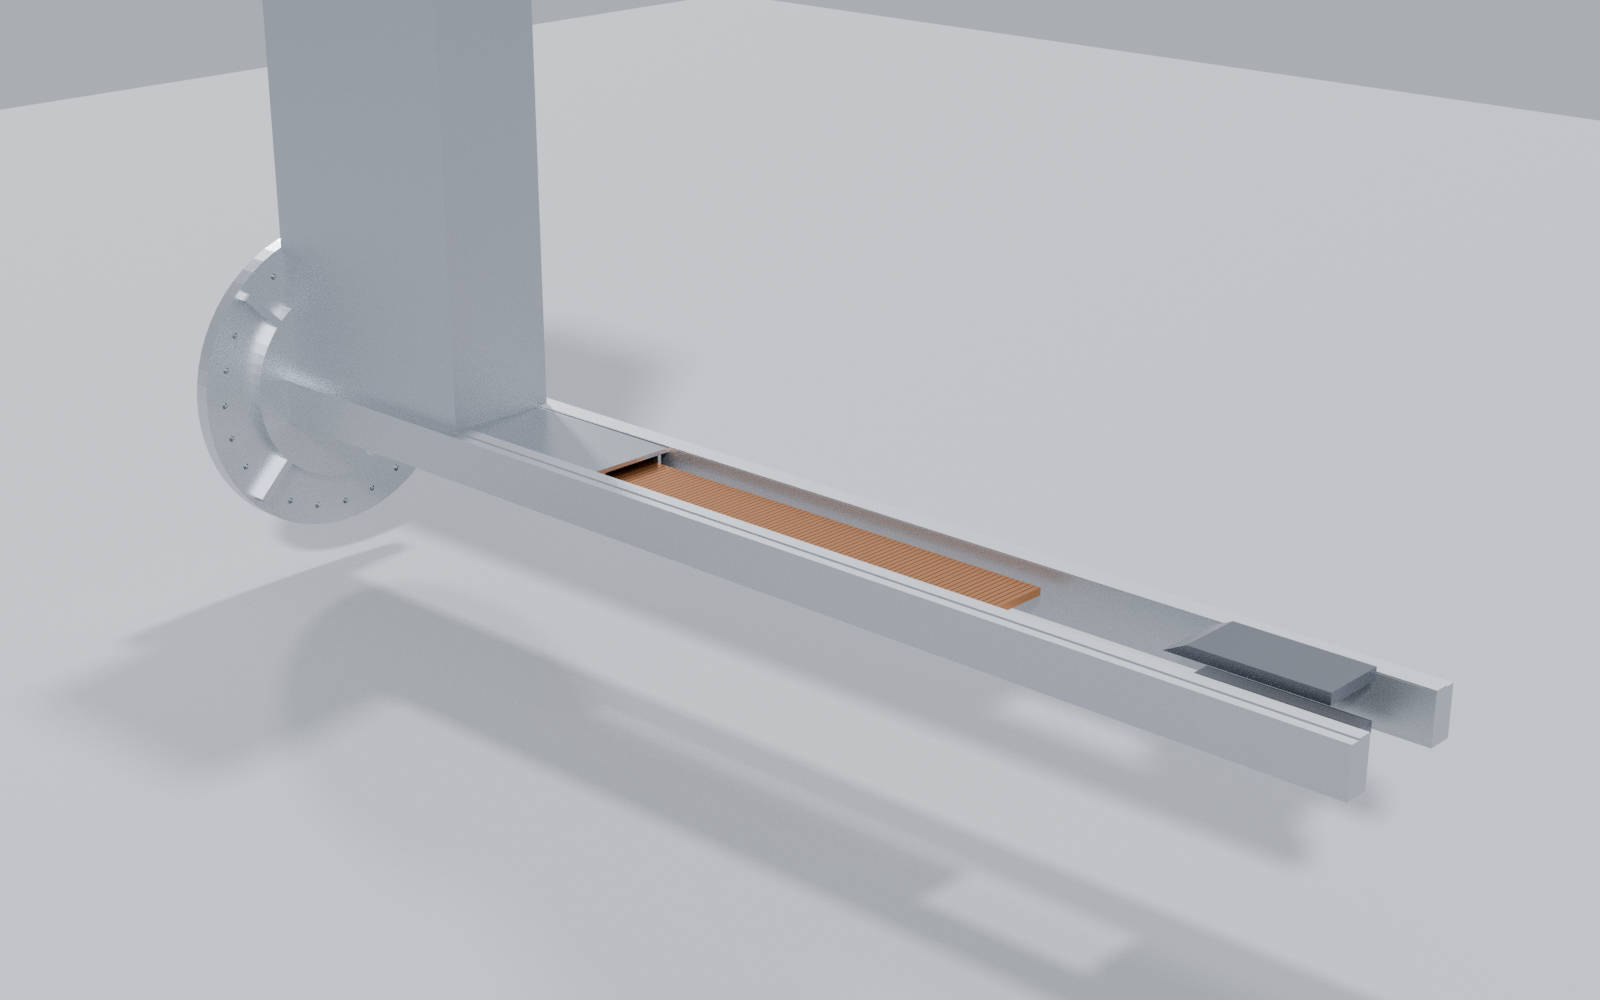
\includegraphics[width=0.84\linewidth,trim=125 205 25 45,clip]{img/hero.png}
\end{center}
\vspace{-1.0mm}
{\scriptsize\textcolor{soft}{\textbf{Gen5 analysed architecture --- CAD model, not flight hardware.}
Ironless double-sided Halbach linear synchronous motor, 1.5\,m track, reusable magnet sled, twelve
3U satellites from two transverse cassettes, contactless eddy-current arrest. Nothing shown here
has been built, fired or measured.}\par}

\vspace{1.8mm}
\shead{The programme, and what each layer is worth}
{\footnotesize
\begin{tabular}{@{}L{24mm}@{\gp}L{38mm}@{\gp}L{\dimexpr\linewidth-70mm\relax}@{}}
\textbf{VOLLEY} & the programme & one question, asked to a fixed evidence standard: can a
propulsion-less satellite be given its own orbit?\\[1.0mm]
\textcolor{ox}{\textbf{Gen5}} & \textcolor{ox}{\textbf{the analysed evidence base}} &
\textcolor{ox}{a self-contained electromagnetic deployer. 65 run sheets, four independent solvers.
\textbf{Everything numeric on this sheet is Gen5.}}\\[1.0mm]
\textbf{Current direction} & stage-integrated, gas-driven & the payload accelerated directly along
a rail a spent upper stage already provides. \textbf{It has not inherited Gen5's validation} and
nothing here is claimed for it.\\
\end{tabular}\par}

\vspace{1.4mm}
\shead{The concept of operations}
\begin{center}
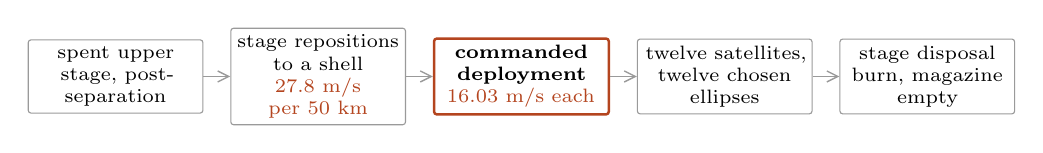
\begin{tikzpicture}[
  font=\scriptsize,
  box/.style={draw=rule,line width=0.4pt,rounded corners=1pt,align=center,inner sep=2.4pt,
              minimum height=8.2mm,text width=20.5mm},
  hot/.style={box,draw=ox,line width=0.9pt},
  a/.style={-{Straight Barb[length=1.4mm,width=1.4mm]},draw=rule,line width=0.5pt}]
\node[box] (s)  {spent upper\\stage, post-\\separation};
\node[box,right=3.4mm of s] (r) {stage repositions\\to a shell\\ \textcolor{ox}{27.8 m/s per 50 km}};
\node[hot,right=3.4mm of r] (d) {\textbf{commanded}\\\textbf{deployment}\\ \textcolor{ox}{16.03 m/s each}};
\node[box,right=3.4mm of d] (o) {twelve satellites,\\twelve chosen\\ellipses};
\node[box,right=3.4mm of o] (x) {stage disposal\\burn, magazine\\empty};
\draw[a] (s)--(r); \draw[a] (r)--(d); \draw[a] (d)--(o); \draw[a] (o)--(x);
\end{tikzpicture}
\end{center}
\vspace{-0.8mm}
{\scriptsize\textcolor{soft}{The host is an active participant, not a mounting surface. A 100\,m/s
host budget reaches four shells and a fleet spanning 269\,km of altitude; plane change is excluded
at 133\,m/s per degree. The altitude half of any multi-orbit claim is bought with host propellant,
not with this machine.}\par}

\vspace{1.4mm}
\shead{Gen5, at the rated point}
{\scriptsize
\begin{tabular}{@{}L{38mm}@{\hspace{2mm}}L{26mm}@{\hspace{7mm}}L{38mm}@{\hspace{2mm}}L{\dimexpr\linewidth-113mm\relax}@{}}
Thrust constant       & \num{10.54} N per kA/m        & Exit velocity, 3U      & \num{16.029} m/s\\
\quad ripple          & $\pm$1.01\,\%                 & \quad acceleration     & \num{10.07}\,$g$ for 162 ms\\
\quad 2-D FEM agrees  & to \num{0.03\,\%}             & Dispersion, closed loop& \num{0.0274} m/s (3$\sigma$)\\
\quad 3-D FEM agrees  & to \num{0.059\,\%}            & \quad as apogee        & $\pm$0.10 km\\[1.2mm]
Energy per shot       & \num{2782} J gross            & Semi-major axis change & \num{+28.8} km\\
\quad net of recovery & \num{2735} J                  & Orbital lifetime       & \num{$\times$1.60} at mean activity\\
\quad to the payload  & 514 J --- \num{18.8\,\%}      & \quad against a spring & +60.2\,\% vs +8.2\,\%\\[1.2mm]
Pulse                 & \num{162.3} ms, 320 A peak    & Mass, dry / loaded     & \num{126.6} / \num{174.6} kg\\
Track first mode      & 109.0 Hz                      & \quad per 3U satellite & \num{10.55} kg\\
Recoil per shot       & 64.1 N$\cdot$s                & Recurring cost         & \num{\rupee\,1{,}345{,}055} --- \emph{every price assumed}\\
\end{tabular}\par}
\vspace{0.8mm}
{\scriptsize\textcolor{soft}{Every figure above is a model output, single-sourced to a committed
JSON result and re-checked against its script on every commit. \textbf{None of it is a measurement,
and no vendor has quoted any line of the cost.}}\par}

\vspace{1.8mm}
\hrulefat\\[1.2mm]
{\footnotesize\textbf{The contribution is the combination, not any one part of it.} Electromagnetic
launch of CubeSats has been studied before, at velocities twenty times higher --- but at
accelerations of order $10^3\,g$ and with a conductive armature bonded to the payload. What is
claimed here is \textbf{a commanded per-satellite velocity, on a satellite that is never modified, at
two orders of magnitude less acceleration, from a stage that was going to be discarded.} Together
they describe a service tier with no demonstrated occupant. \textbf{Whether a given satellite
tolerates 10.07\,$g$ is not claimed}: 25\,$g$ is a ceiling this design sets on itself, no standard
fixes a universal quasi-static limit for CubeSats, and compatibility is a payload-specific
structural question needing an integration review that has not been done.\par}

\newpage
%% ======================================================================
%% BACK
%% ======================================================================
\hrulefat\\[2.0mm]
{\large\bfseries How the numbers were made, and what they cost the argument}\\[1.0mm]
\hrulethin\\[2.0mm]

\shead{The method chain}
{\footnotesize
\begin{tabular}{@{}L{30mm}@{\gp}L{\dimexpr\linewidth-34mm\relax}@{}}
\textbf{Geometry} & Parametric CAD built from one parameter file; 23 dimensions read back out of the model and checked against it.\\
\textbf{Electromagnetics} & Analytic travelling-wave model, cross-checked by \textbf{magpylib}, then by a \textbf{2-D magnetostatic FEM written from the weak form} (scikit-fem, 141\,k elements) to 0.03\,\%, then by a \textbf{3-D reduced-scalar-potential solve} (getdp, 274\,105 DoF) to 0.059\,\%.\\
\textbf{Structures} & \textbf{CalculiX} on the sled chassis and the retention chain.\\
\textbf{Aerodynamics} & \textbf{OpenFOAM} \texttt{simpleFoam} external solve, 581\,779 cells --- for the air correction a ground test would need, not for flight.\\
\textbf{Circuit} & \textbf{ngspice} transient on the pulse chain, against the analytic ledger.\\
\textbf{Astrodynamics} & \textbf{GMAT R2022a} headless, MSISE90, 20$\times$20 gravity, lunisolar and SRP, against this project's own propagator.\\
\textbf{Control} & Closed-loop Monte Carlo, 800 runs, with modelled sensing.\\[1.0mm]
\textcolor{ox}{\textbf{The discipline}} & \textcolor{ox}{\textbf{65 run sheets. Each declares its acceptance bands, and commits them, \emph{before} the script that produces the number exists} --- provable by checking that the band commit touched no script. A failed band moves the design point. \textbf{No band has ever been widened after a result was known.}}\\
\end{tabular}\par}

\vspace{2.0mm}
\shead{What the analysis changed --- the four that cost the most}
{\footnotesize
\begin{tabular}{@{}L{4mm}@{\hspace{2mm}}L{\dimexpr\linewidth-6mm\relax}@{}}
\textbf{1} & \textbf{Exact CAD mass took the headline from 20.37 to 16.029\,m/s.} A parametric 4.86\,kg sled became a 9.445\,kg one when solid volumes were computed; resolving the field through the array's 90\,mm depth, rather than sampling the centre plane, then took another 4.42\,\%. \emph{Both consequences were declared in writing before the analyses ran.}\\[1.0mm]
\textbf{2} & \textbf{An independent propagator falsified a claim in this project's own abstract.} The orbital-lifetime ratio had been offered as invariant across ballistic coefficient and solar activity. GMAT disagreed at low activity by 18\,\% against a 5\,\% band. The cause was the sweep, not the arithmetic: both variables entered the same multiplicative slot, so the ratio could not have moved. \emph{The claim is withdrawn in the manuscript.}\\[1.0mm]
\textbf{3} & \textbf{ngspice found a term no script carried.} Energy closure failed at 97.0\,\% against a declared 98--102\,\%. The missing \textbf{86.6\,J a shot} was the capacitor bank's own series resistance, which the analytic ledger had no term for at all.\\[1.0mm]
\textbf{4} & \textbf{Every kilogram was attributed to the requirement causing it, and then every requirement was deleted.} Across all \textbf{64 corners}, \textbf{88.67\,kg survives} --- 70.06\,\% of dry mass, \textbf{7.39\,kg per satellite against a 2\,kg criterion.} \emph{This is why Gen5 cannot be optimised into its own mass target, and it is the single result that redirected the work.}\\
\end{tabular}\par}

\vspace{1.6mm}
\begin{center}
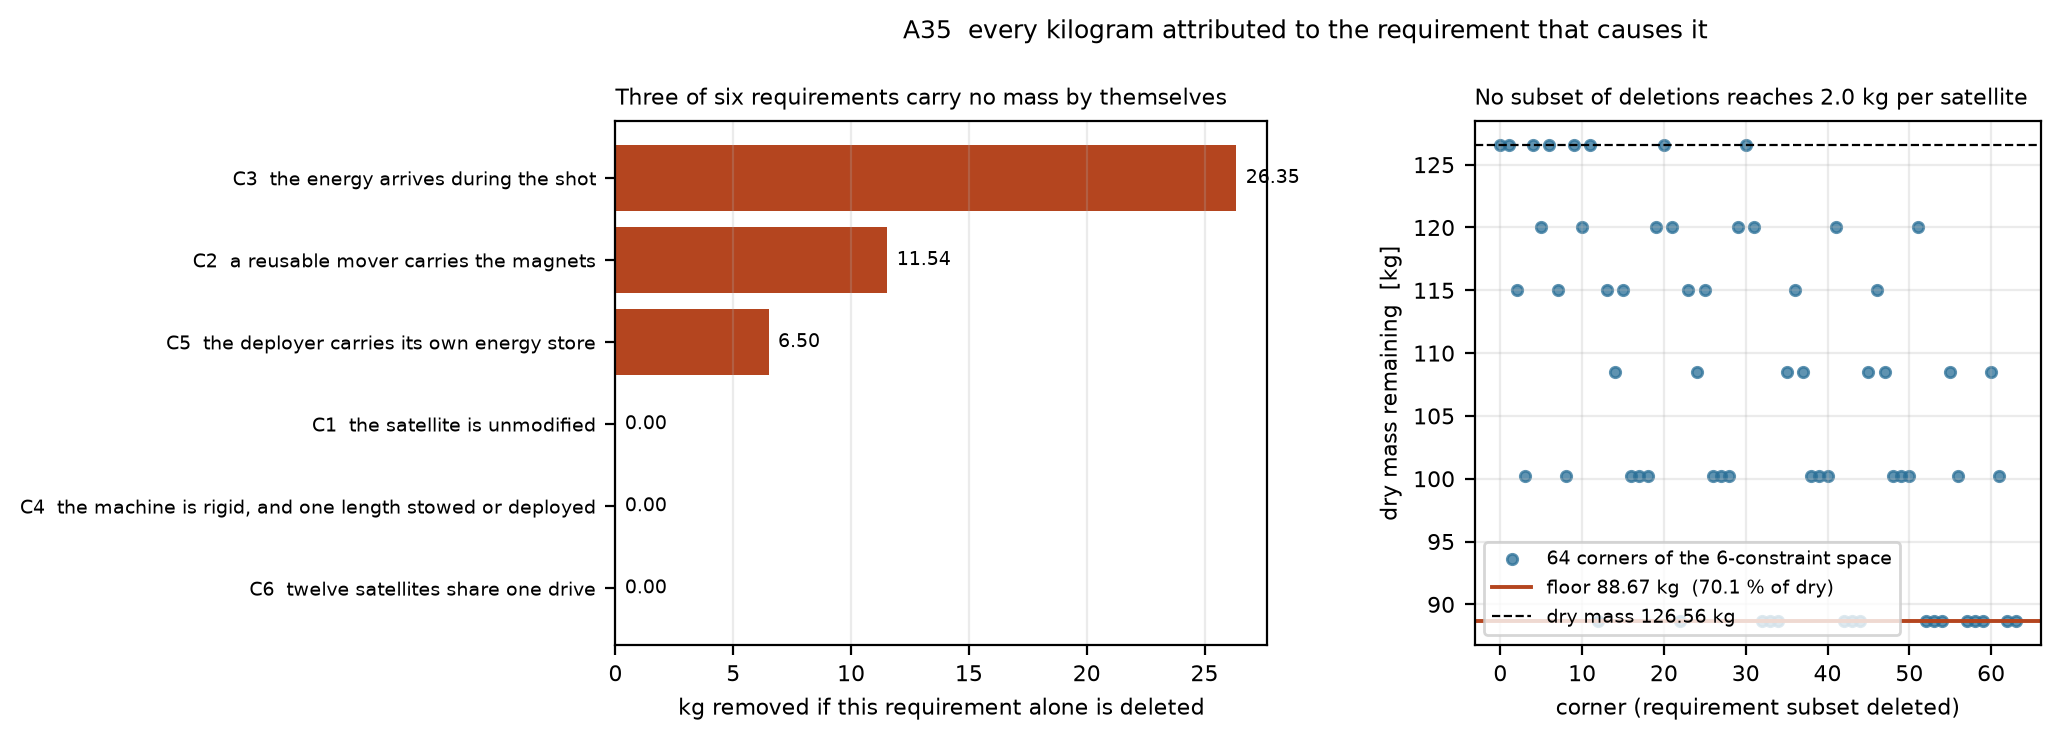
\includegraphics[width=0.485\linewidth]{img/ledger.png}\hfill
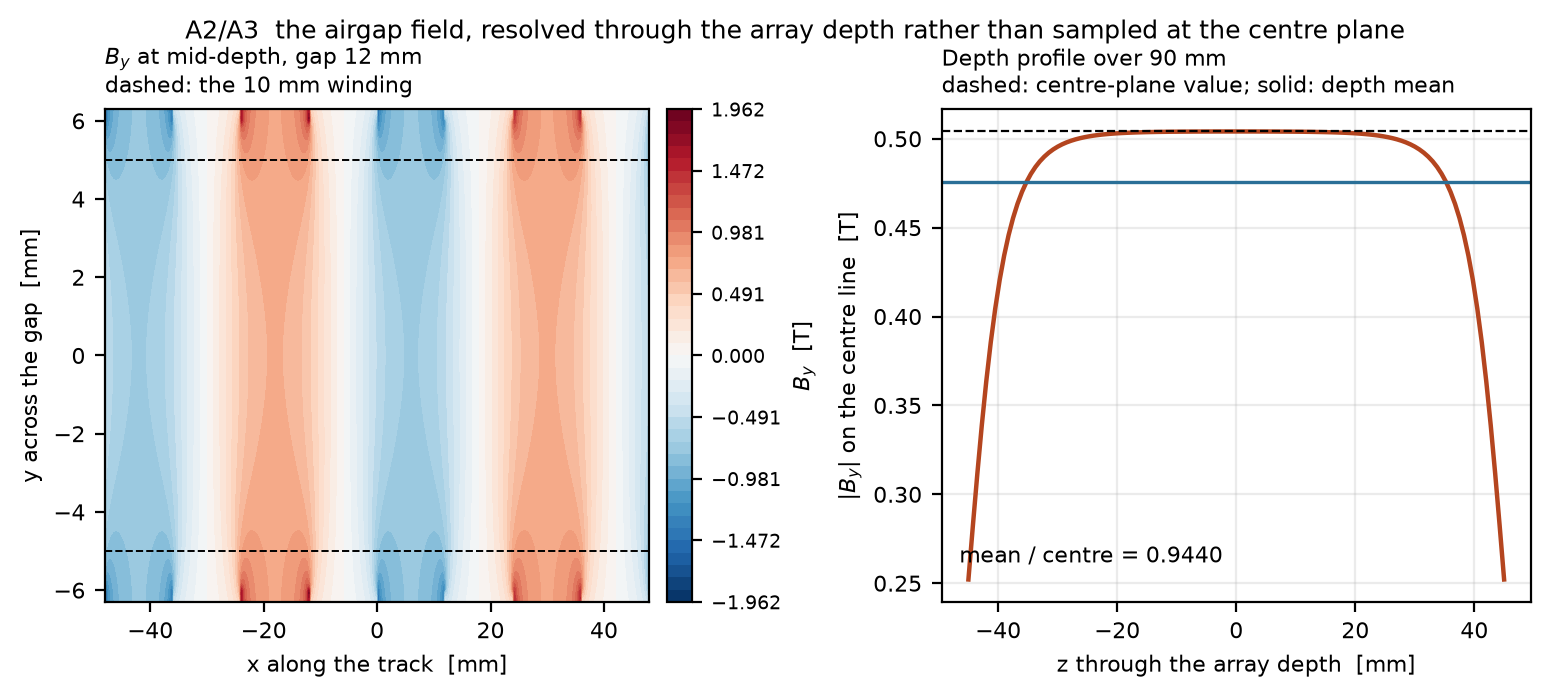
\includegraphics[width=0.485\linewidth]{img/field.png}
\end{center}
\vspace{-1.2mm}
{\scriptsize\textcolor{soft}{Left: the constraint ledger --- what each requirement costs alone, and
the floor no combination of deletions reaches. Right: the airgap field, and the depth profile that
made the thrust constant 4.42\,\% smaller. Both are model outputs.}\par}

\vspace{2.2mm}
\shead{The honest comparison}
{\scriptsize
\begin{tabular}{@{}L{27mm}@{\hspace{3mm}}L{33mm}@{\hspace{3mm}}L{\dimexpr\linewidth-123mm\relax}@{\hspace{3mm}}L{54mm}@{}}
\toprule
 & \textbf{Spring dispenser} & \textcolor{ox}{\textbf{VOLLEY Gen5}} & \textbf{Cold-gas module on the satellite}\\
\midrule
$\Delta v$ per satellite & 1--2.5 m/s, one value for all & \textcolor{ox}{16.03 m/s, commanded} & $\sim$16 m/s\\
Designed differential & \textbf{exactly 0} & \textcolor{ox}{\textbf{16.03 m/s, to 0.027 (3$\sigma$)}} & per satellite\\
Orbital energy & +8.2 \% life at 2.5 m/s & \textcolor{ox}{+28.8 km, $\times$1.60 life} & comparable\\
\textbf{Mass per 3U sat.} & \textbf{$\sim$6.0 kg} & \textbf{10.55 kg --- \emph{loses}, 1.758$\times$} & \textbf{0.5--1.2 kg --- \emph{loses}, 12.4$\times$}\\
Satellite carries & nothing & nothing & pressure vessel, qualification, range safety\\
Host provides & one deploy signal & 150--300 W, serial link, firing window & nothing\\
\textbf{Maturity} & \textbf{TRL 9, thousands flown} & \textbf{TRL 2--3, \emph{nothing measured} --- \emph{loses}}& COTS, flown\\
\bottomrule
\end{tabular}\par}
\vspace{1.0mm}
{\scriptsize\textcolor{soft}{\textbf{Two of the three rows that matter commercially are losses, and
they are printed because they are the result.} Mass parity with a canister of springs was claimed
by this project and is \textbf{withdrawn}: an acceptance band asked for parity within 15\,\% and
the measured ratio is 1.758. So is the constellation-phasing claim --- 30$^\circ$ of in-track phase
costs \textbf{468 seconds of waiting} at zero $\Delta v$, so a spring and a clock reach it and this
machine is not needed for it. \textbf{What survives is the third row: a clock changes phase; a commanded
deployment impulse changes orbital energy.} Drag, $J_2$ and solar pressure change orbits too --- a
clock is not the only thing that cannot. What a clock cannot produce is the \textbf{+28.8\,km of
semi-major axis} a commanded shot does, and no spring at any preload produces it either. No cost comparison is offered in either direction; there is no
quotation for any of it.}\par}

\vspace{2.4mm}
\begin{minipage}[t]{0.70\linewidth}
\shead{Where it goes next}
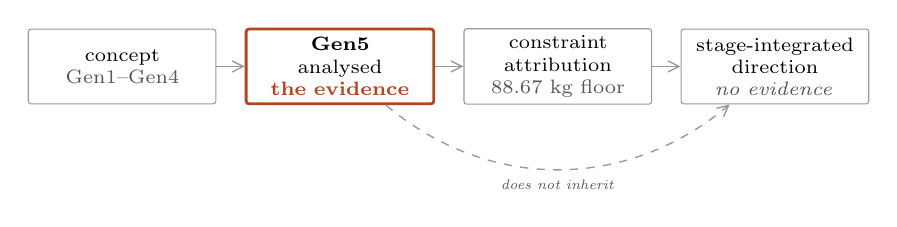
\begin{tikzpicture}[
  font=\scriptsize,
  box/.style={draw=rule,line width=0.4pt,rounded corners=1pt,align=center,inner sep=2.6pt,
              minimum height=9.5mm,text width=22mm},
  ev/.style={box,draw=ox,line width=1.0pt},
  a/.style={-{Straight Barb[length=1.4mm,width=1.4mm]},draw=rule,line width=0.5pt},
  b/.style={-{Straight Barb[length=1.4mm,width=1.4mm]},draw=rule,line width=0.5pt,dashed}]
\node[box] (c) {concept\\ \textcolor{soft}{Gen1--Gen4}};
\node[ev,right=3.6mm of c] (g) {\textbf{Gen5}\\analysed\\ \textcolor{ox}{\textbf{the evidence}}};
\node[box,right=3.6mm of g] (t) {constraint\\attribution\\ \textcolor{soft}{88.67 kg floor}};
\node[box,right=3.6mm of t] (n) {stage-integrated\\direction\\ \textcolor{soft}{\emph{no evidence}}};
\draw[a] (c)--(g); \draw[a] (g)--(t); \draw[a] (t)--(n);
\draw[b] (g) to[out=-40,in=-140] node[below,font=\tiny,text=soft,pos=0.5]{\emph{does not inherit}} (n);
\end{tikzpicture}\\[1.6mm]
{\scriptsize The next step is not more analysis. It is a benchtop track and a mass simulator ---
the point at which the \emph{measured} evidence class in this project's own figure index stops
having zero members.\par}
\end{minipage}\hfill
\begin{minipage}[t]{0.27\linewidth}\raggedleft
\vspace{6.5mm}
\qrcode[height=21mm]{https://github.com/aaaaaaaaaaaavm/VOLLEY}\\[1.4mm]
{\scriptsize\textbf{The full record}\\
\textcolor{soft}{github.com/\\aaaaaaaaaaaavm/VOLLEY}\par}
\end{minipage}

\vspace{2.0mm}
\hrulethin\\[1.2mm]
{\scriptsize\textcolor{soft}{\textbf{Status.} Phase I design study, TRL 2--3. Nothing has been
built, fired, measured, qualified or flown, and no result here has been reviewed by a third party.
Model-to-model agreement between two solvers is a consistency check, not experimental validation.
The defect register carries \textbf{133 numbered entries, 53 of them still open}, including every
one that damages the claims above. \textbf{No institutional, agency or commercial affiliation is
claimed or implied by this document.}}\par}
\end{document}
